%%%%%%%%%%%%%%%%%%%%%%%%%%%%%%%%%%%%%%%%%%%%%%%%%%%%%%%%%%%%%%%%%%%%%%%%%%%%%%%%
% Thesis / Project Report
% LaTeX Template
% Version 2.0 (08/04/16)
%
% Author:
% Aminul
% https://github.com/sidcode/bits-pilani-thesis-
%-------------------------------------------------------------------------------
%	PACKAGES AND OTHER DOCUMENT CONFIGURATIONS
%-------------------------------------------------------------------------------

\documentclass[12pt, a4paper, oneside]{Thesis} % Paper size, default font size
                                               % and one-sided paper
\renewcommand{\bibname}{References}
\graphicspath{{Figures/}} % Specifies the directory where pictures are stored

\usepackage[square, numbers, comma, sort&compress]{natbib}  % Use the "Natbib" style for the references in the Bibliography

\usepackage{verbatim} %for using multi-line comment block

\title{\ttitle} % Defines the thesis title - don't touch this

\begin{document}

\frontmatter % Use roman numbering style (i, ii...) for the pre-content pages

\setstretch{1.3} % Line spacing of 1.3

% Define page headers using FancyHdr package and set up for one-sided printing
\fancyhead{} % Clears all page headers and footers
\rhead{\thepage} % Sets the right side header to show the page number
\lhead{} % Clears the left side page header

\pagestyle{fancy} % Finally, use the "fancy" page style to implement the
                  %FancyHdr headers

% Input all the variables used in the document. Please fill out the
% variables.tex file with all your details.
%-------------------------------------------------------------------------------
%	DOCUMENT VARIABLES
%
%	Fill in the lines below to set the various variables for the document
%-------------------------------------------------------------------------------

%-------------------------------------------------------------------------------
% Your thesis title - this is used in the title and abstract
% Command: \ttitle
\thesistitle{Blackhole Attack Detection In AODV Protocol On VANET}
%-------------------------------------------------------------------------------
% The document type: Thesis / report, etc.
% Command: \doctype
\documenttype{Undergraduate Project}
%-------------------------------------------------------------------------------
% Your supervisor's name - this is used in the title page
% Command: \supname
\supervisor{Md. Rakib Hasan}
%-------------------------------------------------------------------------------
% The supervisor's position - Used on Certificate
% Command: \suppos
\supervisorposition{Lecturer}
%-------------------------------------------------------------------------------
% Supervisor's institute
% Command: \supinst
\supervisorinstitute{Department of Information and Communication Technology\\Comilla University, Cumilla}
%-------------------------------------------------------------------------------
% Your Co-Supervisor's name
% Command: \cosupname
\cosupervisor{Md. Tofael Ahmed}
%-------------------------------------------------------------------------------
% Co-Supervisor's Position - Used on Certificate
% Command: \cosuppos
\cosupervisorposition{Associate Professor}

%-------------------------------------------------------------------------------
% Co-Supervisor's Institute
% Command: \cosupinst
\cosupervisorinstitute{Department of Information and Communication Technology\\Comilla University, Cumilla}
%-------------------------------------------------------------------------------
% Your Examiner's name. Not currently used anywhere.
% Command: \examname
\examiner{}
%-------------------------------------------------------------------------------
% Name of your degree
% Command: \degreename
\degree{Bachelor of Science (Engineering)}
%-------------------------------------------------------------------------------
% The BITS Course Code for which this report is written
% COmmand: \ccode
\coursecode{ICT-800}
%-------------------------------------------------------------------------------
% The name of the Course
% Command: \cname
\coursename{Research Project and Viva}
%-------------------------------------------------------------------------------
% Your name. Extend manually in case of multiple authors
% Command: \authornames
\authors{AMINUL ISLAM TANVIN}
%-------------------------------------------------------------------------------
% Your ID Number - used on the Title page and abstract
% Command: \idnum
\IDNumber{11509015}
%-------------------------------------------------------------------------------
% Your address
% Command: \addressnames
\addresses{}
%-------------------------------------------------------------------------------
% Your subject area
% Command: \subjectname
\subject{}
%-------------------------------------------------------------------------------
% Keywords for this report.
% Command: \keywordnames
\keywords{}
%-------------------------------------------------------------------------------
% University details
% Command: \univname
\university{\texorpdfstring{\href{http://cou.ac.bd/} % URL
                {COMILLA UNIVERSITY, CUMILLA}} % University name
                {COMILLA UNIVERSITY, CUMILLA}}
%-------------------------------------------------------------------------------
% University details, in Capitals
% Command: \UNIVNAME
\UNIVERSITY{\texorpdfstring{\href{http://cou.ac.bd/} % URL
                {COMILLA UNIVERSITY, CUMILLA}} % name in capitals
                {COMILLA UNIVERSITY, CUMILLA}}
%-------------------------------------------------------------------------------
% Department Details
% Command: \deptname
\department{\texorpdfstring{\href{http://cou.ac.bd/ict} % Your department's URL
                {Information and Communication Technology }} % Your department's name
                {Information and Communication Technology}}
%-------------------------------------------------------------------------------
% Department details, in Capitals
% Command: \DEPTNAME
\DEPARTMENT{\texorpdfstring{\href{http://www.bits-pilani.ac.in/pilani/computerscience/ComputerScience} % Your department's URL
                {Information and Communication Technology}} % Your department's name in capitals
                {Information and Communication Technology}}
%-------------------------------------------------------------------------------
% Research Group Details
% Command: \groupname
\group{\texorpdfstring{\href{Research Group Web Site URL Here (include http://)}
                {Research Group Name}} % Your research group's name
                {Research Group Name}}
%-------------------------------------------------------------------------------
% Research Group Details, in Capitals
% Command: \GROUPNAME
\GROUP{\texorpdfstring{\href{Research Group Web Site URL Here (include http://)}
                {RESEARCH GROUP NAME (IN BLOCK CAPITALS)}}
                {RESEARCH GROUP NAME (IN BLOCK CAPITALS)}}
%-------------------------------------------------------------------------------
% Faculty details
% Command: \facname
\faculty{\texorpdfstring{\href{Faculty Web Site URL Here (include http://)}
                {Engineering}}
                {Engineering}}
%-------------------------------------------------------------------------------
% Faculty details, in Capitals
% Command: \FACNAME
\FACULTY{\texorpdfstring{\href{Faculty Web Site URL Here (include http://)}
                {FACULTY NAME (IN BLOCK CAPITALS)}}
                {FACULTY NAME (IN BLOCK CAPITALS)}}
%-------------------------------------------------------------------------------


%-------------------------------------------------------------------------------
%   NON-CONTENT PAGES
%-------------------------------------------------------------------------------
\maketitle
%\Declaration
\Certificate
%
\begin{abstract}
Vehicular mobility is a very important part of the network industry. As the world changed, every wired communication replaced by wireless communication. That's why VANET is very important. For being wireless it has lots of facilities. Also, have some drawbacks about the security issue. This type of network is affected by network attack like blackhole attack. Without taking steps against this issue the vanet is not reliable. A new blackhole attack detection technique is proposed which uses AODV as routing protocol. It detects the blackhole nodes and sends the information to the admin of the network. We also compare the blackhole attack with a flawless network.

\end{abstract}

\begin{acknowledgements}

At first, I want to express gratitude to the Almighty Allah for His endless kindness for keeping me mentally and physically fit to complete this sophisticated task.

I would like to express my special thanks of gratitude to my honorable supervisor   Md. Rakib Hasan, who gave me the golden opportunity to do this wonderful project on this topic. His sage advice, insightful criticisms, and patient encouragement aided the completion of this project in innumerable ways. I came to know about so many new things, I am greatly thankful to him.

I am also thankful to \cosupervisor, Head of Department, \cosupervisorinstitute for the motivation and inspiration that triggered me for this thesis work.

I would like to express my gratitude to all the teachers in my department for building me to do this work.


\end{acknowledgements}





%-------------------------------------------------------------------------------
%	LIST OF CONTENTS/FIGURES/TABLES PAGES
%-------------------------------------------------------------------------------


% The page style headers have been "empty" all this time, now use the "fancy"
% headers as defined before to bring them back
\pagestyle{fancy}

\lhead{\emph{Contents}} % Set the left side page header to "Contents"
\tableofcontents % Write out the Table of Contents

% Set the left side page header to "List of Figures"
\lhead{\emph{List of Figures}}
\listoffigures % Write out the List of Figures

% Set the left side page header to "List of Tables"
\lhead{\emph{List of Tables}}
\listoftables % Write out the List of Tables
\clearpage  % Start a new page
\lhead{\emph{LIST OF ABBREVIATION }}  % Set the left side page header to "Abbreviations"
\listofsymbols{ll}  % Include a list of Abbreviations (a table of two columns)
{
% \textbf{Acronym} & \textbf{W}hat (it) \textbf{S}tands \textbf{F}or \\
\textbf{NetAnim} & \textbf{NET}work \textbf{ANIM}ator \\

\textbf{VANET} & \textbf{V}ehicular \textbf{A}d-hoc \textbf{NET}work  \\

\textbf{AODV} & \textbf{A}d-hoc \textbf{O}n-Demand \textbf{D}istance  \textbf{V}ector  \\

\textbf{RREQ} & \textbf{R}outing \textbf{REQ}uest \\

\textbf{SUMO} & \textbf{S}imulation of \textbf{U}rban \textbf{MO}bility \\

\textbf{NS2} & \textbf{N}etwork \textbf{S}imulator \textbf{2}  \\

\textbf{IDS} & \textbf{I}ntrusion \textbf{D}etection \textbf{S}ystem  \\

\textbf{IPS} & \textbf{I}ntrusion \textbf{P}revention \textbf{S}ystem  \\

\textbf{OSM} & \textbf{O}pen \textbf{S}treet \textbf{M}ap  \\
}

\clearpage
%% ----------------------------------------------------------------


%-------------------------------------------------------------------------------
%	THESIS CONTENT - CHAPTERS
%-------------------------------------------------------------------------------

\mainmatter % Begin numeric (1,2,3...) page numbering

\pagestyle{fancy} % Return the page headers back to the "fancy" style

% Include the chapters of the thesis as separate files from the Chapters folder
% Uncomment the lines as you write the chapters

% Chapter 1

\chapter{Introduction} % Main chapter title

\label{Chapter1} % For referencing the chapter elsewhere, use \ref{Chapter1}

\lhead{Chapter 1. \emph{Introduction}} % This is for the header on each page - perhaps a shortened title
Bangladesh has a very high road accident fatality rate. Every day around eight per-
sons die in road accidents.\cite{qn} So road security is the main issue for now. To trade off with traffic accidents and vehicle speed we have to develop new road technology. That's why VANET is important now a day.

\section{Introduction}
A Vehicular Ad hoc Network (VANET) is a form of wireless ad-hoc network to
provide communications among vehicles and nearby roadside equipment. It is
emerging as a new technology to integrate the capabilities of a new generation
wireless networking to vehicles. The major purpose of VANET is to provide
(1) ubiquitous connectivity while on the road to mobile users, who are otherwise
connected to the outside world through other networks at home or the work
place, and (2) efficient vehicle-to-vehicle communications that enable the Intelligent Transportation Systems (ITS). ITS includes a variety of applications such
as cooperative traffic monitoring, control of traffic flows, blind crossing
(a crossing without light control), prevention of collisions, nearby information
services, and real-time detour routes computation.


\section{Motivation}
Bangladesh is the 12th most densely settled nation on earth. The traffic jam is the most threat
to developing countries like Bangladesh. Only Dhaka's traffic jams eat up 3.2 million working hours each day and drain billions of dollars from the city's economy annually. So it is important to develop a new international standard on the road. That is not other than VANET.
When a new technology is evolved the security is the main concern. The intruder uses the technology to threaten the improvement. To improve network-level security we work for network layer attack (blackhole). 
This blackhole attack detection helps us to improve the infrastructure of our
road and vehicle.\cite{qn}
\\\\
There are not enough routes to transport the metropolis's 17 million-plus residents.
For being a member of this country it is a job to think about the problem of this country
and try to solve them.
\section{Rationale of the Study}

In this research, simulation of a network layer attack(blackhole) is done using NS2 as a simulator.
Blackhole attack is a denial of service attack where a malicious node pretends to be the first
hop for the shortest path. When the packet is sent to the blackhole node it drops the packet
instead of sending the packet to the next hop. In vanet, it is hard to define a node as blackhole
because many legitimate node drop packet(s) for proper reason.\\\\ VANET is a figureless topology.
That's why the node(s) are not stable in one place, so the malicious node could be change location and pretend to be a legitimate node. Blackhole nodes have to be blocked by the MAC address.


\section{Research Questions}
The research questions for this study were:\\\\
1. How to Detect malicious node(s) in Blackhole attack on VANET?\\\\
2. Is this approach efficient to use in blackhole attack?\\\\
3. Can we use this model in our real life ?\\\\


\section{Expected Output}

Simulation of 50 nodes vehicular ad-hoc network by using ns2 is performed.
In TCL file we make some nodes as malicious and see the output by the network protocol that modified to detect the blackhole node by using the predefined variable in the TCL file of the corresponding node. The detecting output shows in the terminal window. The effect of the attack is stored in the trace file. Simulation can be shown in animation using netanim.
\section{Report Layout}

This report is divided into 5 chapters and they are\\ 
Chapter \ref{Chapter1}: {Introduction} \\
 Chapter \ref{Chapter2}: {Background} \\ 
 Chapter \ref{Chapter3}: {Research Methodology} \\ 
 Chapter \ref{Chapter4}: {Experimental Results and Discussion}\\
  Chapter \ref{Chapter5}: {Conclusion and Implication for Future}\\
At the end of the paper, we add References and Appendices  \\ Abstract is placed at the very first of the paper.
\\\\

% Chapter 2

\chapter{Background} % Main chapter title

\label{Chapter2} % For referencing the chapter elsewhere, use \ref{Chapter2}

\lhead{Chapter 2. \emph{Background}} % This is for the header on each page - perhaps a shortened title

%----------------------------------------------------------------------------------------
\section{Introduction}
VANET is a kind of MANET with vehicular node.
Traffic has a great impact on the economy of the 21st century. For the safer and flawless network on the road, we have to use a better protocol and some applications like IDS, IPS.

\section{Related Works}
H. Deng et al.\cite{qa:1} discussed a protocol that requires intermediate nodes for sending RREP message along with the next-hop information. When the source node gets this information,
it sends an RREQ to the next hop to verify that the target node indeed has a route to the intermediate node and the destination. When
the next hop receives a Further Request, it sends a Further
Reply which includes the check result to the source node.
Based on information in Further Reply, the source node judges
the validity of the route. In this protocol, the RREP control
packet is modified to contain the information about next-hop.
After receiving RREP, the source node will again send RREQ
to the node specified as next hop in the received RREP.\\\\

B. Sun et al. \cite{qa:2} use AODV as their routing protocol and
simulation is done in the ns2 simulator. The detection technique
is a neighborhood-based method to detect the black hole
attack and then present a routing recovery protocol to build the
the real path to the destination. Based on the neighbor set
information, a method is improved to deal with the black hole
attack. Source node
sends a modify-Route-Entry (MRE) control packet to the
Destination node to form a correct path by modifying the
routing entries of the intermediate nodes (IM) from source to
destination.\\\\

S. Ramaswamy et al. presented an algorithm in \cite{qa:3} which
claims to prevent the black hole attacks in ad-hoc
network. In this algorithm each node maintains additional data packets, a node must show its honesty. If a node is the
first receiver of an RREP packet, it forwards packets to source
and initiates the judgment process on about replier. The judgment
process depended on the opinion of the network’s nodes about
replier. These neighbors are requested to send their opinion
about a node. When a node collects all opinions of neighbors,
it decides if the replier is a malicious node based on number
rules.\\\\

M.Y. Su \cite{qa:4} proposed the mechanism to detect and separate
malicious nodes, which selectively perform black hole attacks
by deploying IDSs in MANETs (mobile ad hoc networks). All
IDS nodes perform an ABM (Anti-Black hole Mechanism),
which estimates the suspicious value of a node, according to
the amount of abnormal difference between RREQs and
RREPs transmitted from the node. With the prerequisite that
intermediate nodes are forbidden to reply to RREQs if an
intermediate node, which is not the destination and never
broadcasts an RREQ for a specific route, forwards an RREP for
the route, then its suspicious value will be increased by 1 in
the nearby IDS’s SN (suspicious node) table. When the
suspicious value of a node exceeds a threshold, a Block
message is broadcasted by the detected IDS to all nodes on the
network to cooperatively isolate the suspicious node.\\\\

Some attempts have been made for securing wireless monile communication, such as: Secure Efficient Ad hoc Distance vector
routing protocol (SEAD) \cite{qa:5}, the secure on-demand routing
protocol - Ariadne \cite{qa:6}, authenticated routing for ad hoc
networks (ARAN)  \cite{qa:7}, Security-aware ad hoc routing (SAAR)
\cite{qa:8}, Resiliency Oriented Secure (ROS)  \cite{qa:9}, Secure Routing
Protocol (SRP)  \cite{qa:10}, Secure AODV (SAODV)  \cite{qa:11}, Secure Link-
State Protocol (SLSP)  \cite{qa:12}, Cooperative Security-Enforcement
Routing (CSER)  \cite{qa:13}

\section{Research Summary}

A solution is proposed to identify a black hole
node, remove that node from the routing table and finally added to
the blacklist table.
The layout of the network is given below.
%Figure   
\begin{figure}[htbp]
	\centering
	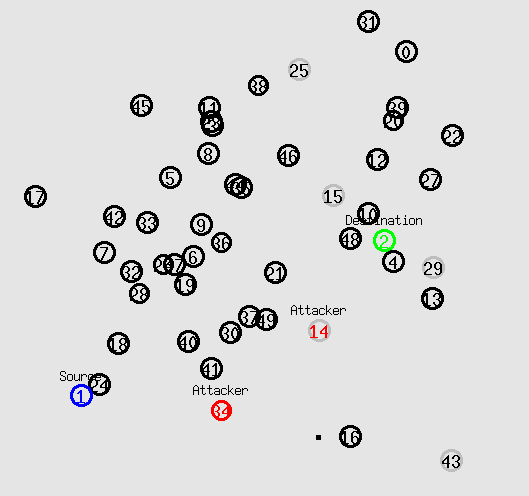
\includegraphics[scale=.5]{black2}
	\rule{35em}{0.5pt}
	\caption[Layout of network]{Layout of Network}
	\label{fig:layout}
\end{figure}


\section{Scope of the Problem}

The purpose of the work is to make a secured network where the blackhole attacker is detected and marked as a malicious node. 50 noded network is used in this study and make 3 of them as malicious. Whenever they drop the packet from a legitimate node. The simulation is run 8 min and Sent total 616 packet \\
To detect the malicious node we had slightly
enhanced the AODV protocol working. In our approach, when
the sender broadcasts the RREQ packet, it will wait for reply.
If the hop count is very short every time then the node is marked as a malicious node.

\section{Challenges}

Vehicular ad-hoc network is a self-composing network with a highly dynamic network topology. For its dynamicity, though
it has many advantages it faces some safety issues. That fall it in threat. If we can fix those issues, VANET can be use
heedlessly.\\
For the Exporting graph from the trace file, there is no much available application. We used a very old software named
tracegraph.\\
Vanet is complex compared to other mobility networks.

% Chapter 3

\chapter{Research Methodology} % Main chapter title

\label{Chapter3} % For referencing the chapter elsewhere, use \ref{Chapter3} 

\lhead{Chapter 3. \emph{Research Methodology}} % This is for the header on each page - perhaps a shortened title

%----------------------------------------------------------------------------------------
In this work,  the aodv protocol slightly enhanced for making this protocol to detect blackhole node. Have to add some extra code in the header file of the protocol. The routing table and receive request is modified for this system build.



\section{Introduction}

Blackhole node is detected by this system. and information about detection is sent in the terminal. Admin may block this particular node from this network.\\
AODV protocol depends on some header files. we should have configured those files also.
%Figure   
\begin{figure}[htbp]
	\centering
	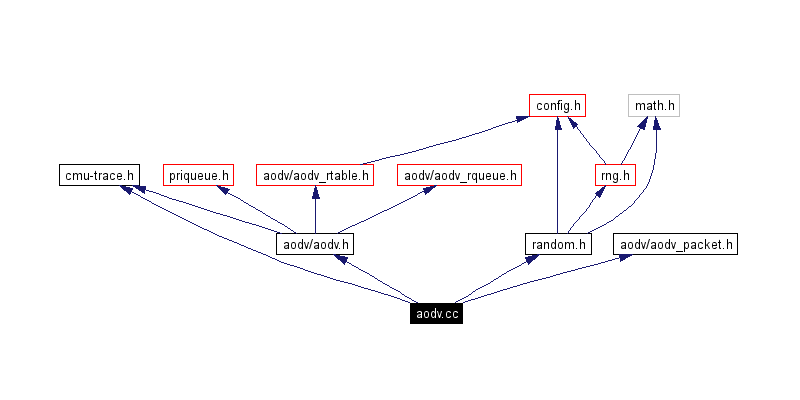
\includegraphics[scale=0.4]{aodv1}
	\rule{35em}{0.5pt}
	\caption[Dependencies of aodv.cc]{Dependencies of aodv.cc}
	\label{Dependencies of aodv.cc}
\end{figure}
\pagebreak
In this project, the nature of the blackhole attack is used to detect the blackhole node.
The main purpose of this work to detect malicious node in a crowded road where the blackhole mislead us in a wrong road where there is a barricade or the road is blocked.

%Figure   
\begin{figure}[htbp]
	\centering
	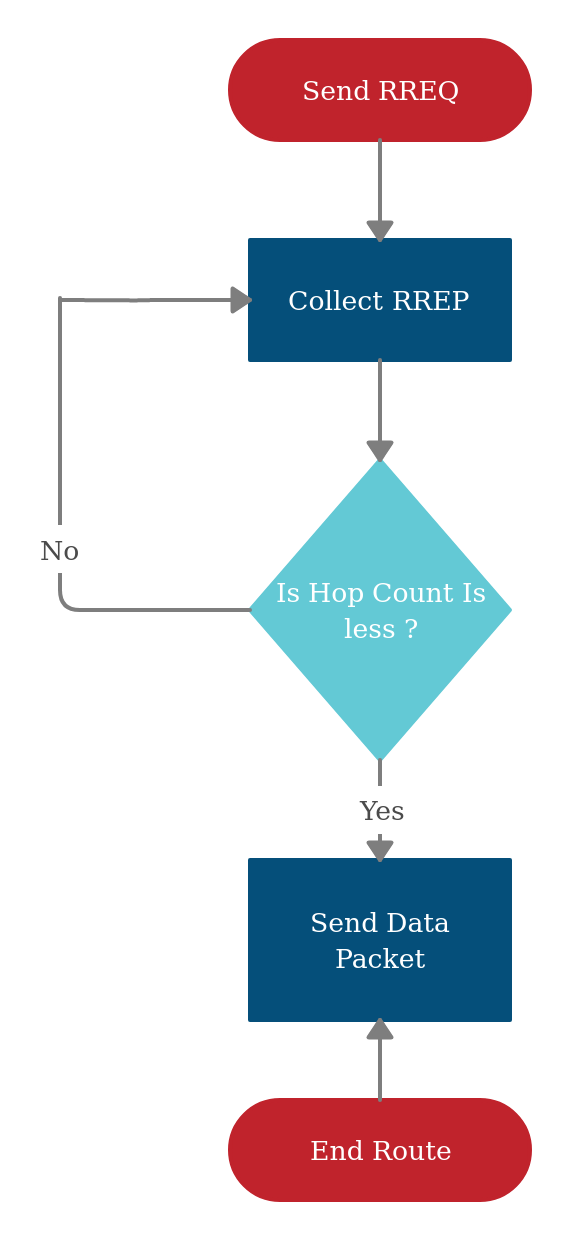
\includegraphics[scale=0.2]{algorithm}
	\rule{35em}{0.5pt}
	\caption[Algorithm Of Work]{Work Flow}
	\label{flow}
\end{figure}

\section{Research Subject and Instrumentation}

First of all, A VANET is created using OSM. This file is used as a source of the TCL file of the network that takes up from the ns2 package. The TCL file is used to mark a node as malicious. After that, aodv.cc and aodv.h is edited to implement the main detection algorithm. \\\\
In Blacklist table, each node will check its table to identify
whether the packet is coming from the malicious node. If this is
true, it will discard the packet. Also when any node identifies
the malicious node, it will send alarm packets to the entire
network about the malicious behaviors of the node thereby
removing the node from the routing table and adding it in the
blacklist table.

\subsection{SUMO}
Sumo is an application to generate a vanet network. we use two tools of sumo application and they are \\
1. osm web wizerd\\
2.trace exporter\\\\
osmWebWizerd is used to get real-time data from the map and generate a network scenario. After that, we use trace exporter to convert this scenario to a trace file.


\subsection{NS2}
It is a discrete-time simulator. The designed protocol can be applied in it. NS2 is a mostly used open-source simulation application. \\
Though there is a new version of ns named ns3, the older version is used because of having efficient knowledge in ns2.
\subsection{Tracegraph}
The trace file is analyzed with tracegraph. Two trace file (with malicious node, without malicious node) is created, observing both files and see the difference in between them. Three parameter is used in this project.

\section{Data Collection Procedure}
Auto-generated traffic mobility data is created with sumo application.
It auto-generates in real-world locations and has information about authentic data. It uses python package as it's design.

%Figure   
\begin{figure}[htbp]
	\centering
	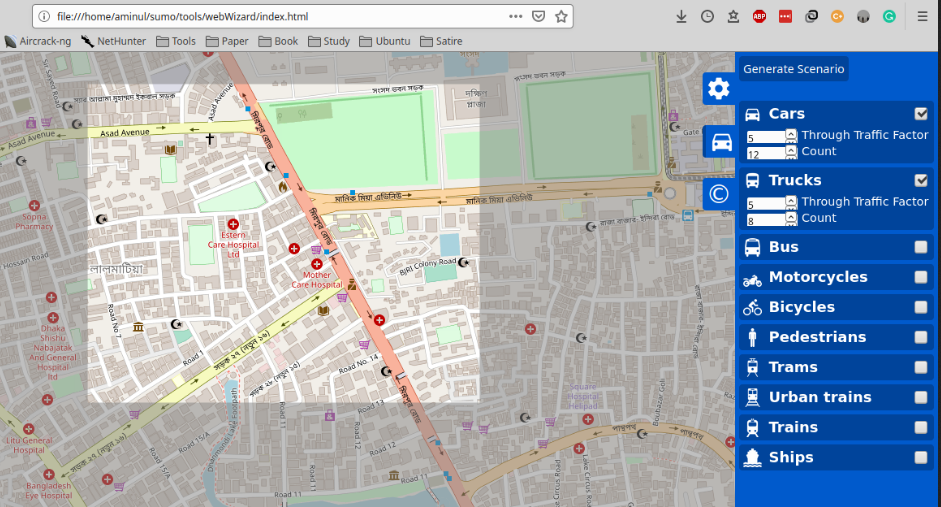
\includegraphics[scale=0.5]{sumo}
	\rule{35em}{0.5pt}
	\caption[Data Collection]{Data Collection}
	\label{Data Collection}
\end{figure}

\pagebreak
\section{Implementation Requirements}
Requirements of this project are \\
1. Basic command of the Linux operating system.\\
2. Clear idea about network and routing.\\
3. NS2 is the simulation application. Have to have an idea about build and change routing code of it.\\
4. analyzation of simulation performed using tracegraph. Basic parameter of a network like throughput, jitter cumulative sum, etc.\\
5. All ns2 code is written in C++. Have to have the ability to understand those code.
% Chapter 4

\chapter{Experimental Results and Discussion} % Main chapter title

\label{Chapter4} % For referencing the chapter elsewhere, use \ref{Chapter3} 

\lhead{Chapter 4. \emph{Results}} % This is for the header on each page - perhaps a shortened title

%----------------------------------------------------------------------------------------
Malicious nodes detected properly by this simulation. When a blackhole node drops a packet the IDS detects the blackhole and gives output in the terminal.[\ref{fig:terminal}] And send the malicious node to the blacklist.

\section{Introduction}

In this simulation, blackhole node is detected in ns2. AODV is a reactive routing protocol. When the source node searches the route for communication. It sends RREQ to the neighbor nodes and sends the RREP to the route 1st hop. If 1st node drops the packet the message is sent to the admin that which node drop whose packet. A comparison between with and without blackhole is given in the table. \ref{tab:compare}

\begin{table}[]
	\centering
	\begin{tabular}{|l|l|l|}
		\hline
		\textbf{Parameter}          & \textbf{With Blackhole} & \textbf{Without Blackhole} \\ \hline
		Simulation  time in seconds & 7.969744514             & 7.996721981                \\ \hline
		Number of nodes             & 50                      & 50                         \\ \hline
		Number of sent packets      & 679                     & 1148                       \\ \hline
		Number of dropped packets   & 693                     & 616                        \\ \hline
		Average packet size         & 63.6649                 & 83.0259                    \\ \hline
		Number of dropped bytes     & 82048                   &           66566              \\ \hline
	\end{tabular}
	\caption{Simulation Comparison Of Blackhole Attack}
	\label{tab:compare}
\end{table}

%Figure   
\begin{figure}[htbp]
	\centering
	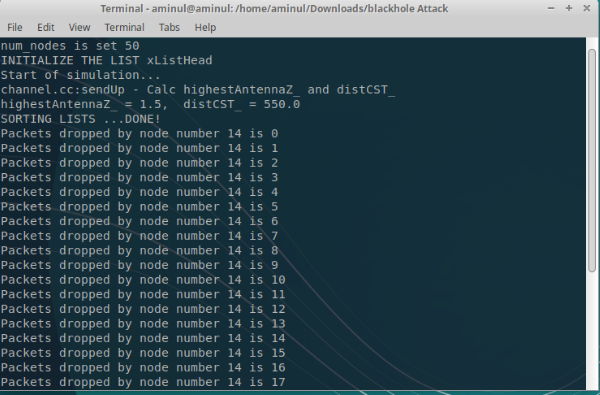
\includegraphics[scale=0.5]{out}
	\rule{35em}{0.5pt}
	\caption[Output in terminal]{Output in terminal}
	\label{fig:terminal}
\end{figure}
\pagebreak
\section{Experimental Results}
In this simulation 50 nodes is used and this simulation took place for around 8 min.
Both with and without blackhole nodes the simulation performed and observed the output.
It is observed that when the blackhole nodes are presented packet was sent in huge in number and drop rate is also higher. Throughput of generated packets are decreases almost 50\% less with 3 blackhole nodes among 50 nodes.\\

Three parameters are considered in this simulation.
They are:\\
1.Cumulative Sum\\
2.Throughput\\
3.Jitter
\subsection{Cumulative Sum}
It is a sequential analysis process. It is used to monitoring change detection. In a network, cumulative sum indicates the use of the network. when the malicious node is present the traffic of the network increases so the cumulative sum increased. \cite{gao2020cumulative}

% Please add the following required packages to your document preamble:
% \usepackage{multirow}
\begin{table}[]
	\begin{tabular}{|c|l|l|l|}
		\hline
		\textbf{Parameter}                 & \textbf{Nature} & \textbf{With Blackhole} & \textbf{Without Blackhole} \\ \hline
		\multirow{3}{*}{generated packets} & Minimum         & 1.00                    & 1.00                       \\ \cline{2-4}
		& Average         & 374.50                  & 583.50                     \\ \cline{2-4}
		& Maximum         & 748.00                  & 1166.00                    \\ \hline
		\multirow{3}{*}{sent packets}      & Minimum         & 1.00                    & 1.00                       \\ \cline{2-4}
		& Average         & 315.00                  & 560.50                     \\ \cline{2-4}
		& Maximum         & 629.00                  & 1120.00                    \\ \hline
		\multirow{3}{*}{forwarded packets} & Minimum         & 1.00                    & 1.00                       \\ \cline{2-4}
		& Average         & 19.50                   & 71.50                      \\ \cline{2-4}
		& Maximum         & 38.00                   & 142.00                     \\ \hline
		\multirow{3}{*}{received packets}  & Minimum         & 1.00                    & 1.00                       \\ \cline{2-4}
		& Average         & 630.00                  & 522.50                     \\ \cline{2-4}
		& Maximum         & 1259.00                 & 1044.00                    \\ \hline
		\multirow{3}{*}{dropped packets}   & Minimum         & 1.00                    & 1.00                       \\ \cline{2-4}
		& Average         & 347.00                  & 308.50                     \\ \cline{2-4}
		& Maximum         & 693.00                  & 616.00                     \\ \hline
	\end{tabular}
	\caption{Cumulative Sum Of Dropped Packets Simulation}
	\label{tab:sum}
\end{table}

%Figure   
\begin{figure}[htbp]
	\centering
	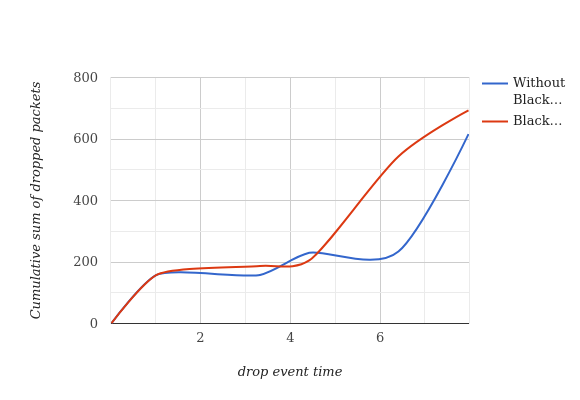
\includegraphics[scale=0.5]{sum}
	\rule{35em}{0.5pt}
	\caption[Cumulative sum of dropped packets]{Cumulative sum of dropped packets}
	\label{fig:sum}
\end{figure}


\subsection{Throughput}
It is a transmission measurement parameter. It is a ratio of transmitted traffic and unit of time. It is the best way of measuring a network. If the throughput is higher the traffic of the network is more. We should avoid a system with high traffic.

% Please add the following required packages to your document preamble:
% \usepackage{multirow}
\begin{table}[]
	\begin{tabular}{|c|l|l|l|}
		\hline
		\textbf{Parameter}                 & \textbf{Nature} & \textbf{With Blackhole} & \textbf{Without Blackhole} \\ \hline
		\multirow{3}{*}{generated packets} & Minimum         & 1.00                    & 1.00                       \\ \cline{2-4}
		& Average         & 83.11                   & 129.55                     \\ \cline{2-4}
		& Maximum         & 220.00                  & 220.00                     \\ \hline
		\multirow{3}{*}{sent packets}      & Minimum         & 1.00                    & 1.00                       \\ \cline{2-4}
		& Average         & 69.89                   & 124.44                     \\ \cline{2-4}
		& Maximum         & 165.00                  & 198.00                     \\ \hline
		\multirow{3}{*}{forwarded packets} & Minimum         & 0.00                    & 1.00                       \\ \cline{2-4}
		& Average         & 4.22                    & 15.78                      \\ \cline{2-4}
		& Maximum         & 17.00                   & 20.00                      \\ \hline
		\multirow{3}{*}{received packets}  & Minimum         & 1.00                    & 1.00                       \\ \cline{2-4}
		& Average         & 139.89                  & 116.00                     \\ \cline{2-4}
		& Maximum         & 256.00                  & 231.00                     \\ \hline
		\multirow{3}{*}{dropped packets}   & Minimum         & 1.00                    & 0.00                       \\ \cline{2-4}
		& Average         & 77.00                   & 68.44                      \\ \cline{2-4}
		& Maximum         & 204.00                  & 213.00                     \\ \hline
	\end{tabular}
	\caption{Throughput Of Dropping Packets Simulation}
	\label{tab:through}
\end{table}

%Figure   
\begin{figure}[htbp]
	\centering
	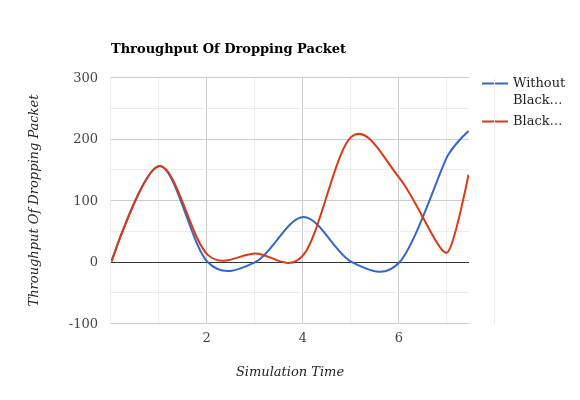
\includegraphics[scale=0.5]{through}
	\rule{35em}{0.5pt}
	\caption[Throughput Of Dropping Packet]{Throughput Of Dropping Packet}
	\label{Throughput Of Dropping Packet}
\end{figure}


\subsection{Jitter}
It is the variance in the time delay between a data packet over a network. It is defined as to disturb in normal packet sending sequence. Jitter helps in decision making about a network.


% Please add the following required packages to your document preamble:
% \usepackage{multirow}
\begin{table}[]
	\begin{tabular}{|c|l|l|l|}
		\hline
		\textbf{Parameter}                 & \textbf{Nature} & \textbf{With Blackhole} & \textbf{Without Blackhole} \\ \hline
		\multirow{3}{*}{generated packets} & Minimum         & -0.01                   & -0.01                      \\ \cline{2-4}
		& Average         & 0.11                    & 0.045                      \\ \cline{2-4}
		& Maximum         & 0.29                    & 0.28                       \\ \hline
		\multirow{3}{*}{sent packets}      & Minimum         & -0.01                   & -0.01                      \\ \cline{2-4}
		& Average         & 0.11                    & 0.04                       \\ \cline{2-4}
		& Maximum         & 0.29                    & 0.28                       \\ \hline
		\multirow{3}{*}{forwarded packets} & Minimum         & -0.01                   & -0.01                      \\ \cline{2-4}
		& Average         & 0.11                    & 0.05                       \\ \cline{2-4}
		& Maximum         & 0.28                    & 0.28                       \\ \hline
		\multirow{3}{*}{received packets}  & Minimum         & 0.01                    & 0.01                       \\ \cline{2-4}
		& Average         & 0.15                    & 0.20                       \\ \cline{2-4}
		& Maximum         & 0.37                    & 0.37                       \\ \hline
		\multirow{3}{*}{dropped packets}   & Minimum         & 0.00                    & 0.00                       \\ \cline{2-4}
		& Average         & 0.10                    & 0.14                       \\ \cline{2-4}
		& Maximum         & 0.40                    & 0.38                       \\ \hline
	\end{tabular}
	\caption{Jitter Of Dropped Packets Simulation}
	\label{tab:jitter}
\end{table}

%Figure   
\begin{figure}[htbp]
	\centering
	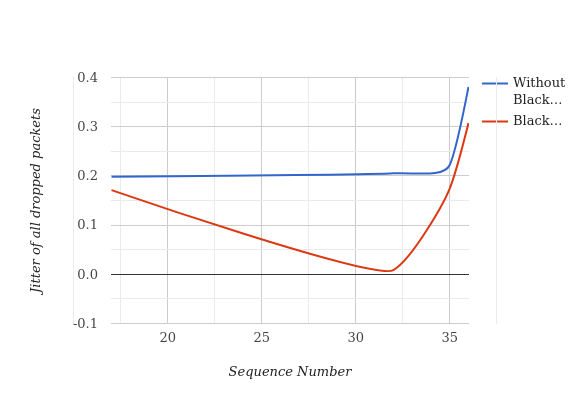
\includegraphics[scale=0.5]{jitter}
	\rule{35em}{0.5pt}
	\caption[Jitter Of Dropped Packets]{Jitter of dropped packets}
	\label{fig:jitter}
\end{figure}
\pagebreak\
\section{Descriptive Analysis}
50 nodes simulation when 3 of them are blackhole is observed. In this process of identification every node is observed. The network size doesn't matter in this case. Ad-hoc on demand routing is most used and efficient routing protocol. It is secured in nature. Result of this project is satisfectory.


\section{Summary}
It observed that the cumulative sum of packet dropping increases 12.66\% for 3 malicious nodes.\\At same way throughput of dropping packet increase by 12.51 \% \& average jitter of dropping a packet is increased by 40\%.
% Chapter 5

\chapter{Conclusion and Implication for Future} % Main chapter title

\label{Chapter5} % For referencing the chapter elsewhere, use \ref{Chapter3} 

\lhead{Chapter 5. \emph{Conclusion and Implication for Future}} % This is for the header on each page - perhaps a shortened title

%----------------------------------------------------------------------------------------
\section{Summary of the Study}

This simulation is based on blackhole attack detection in a vanet when aodv is using as a routing protocol. Vanet is used in the vehicle so it has a huge impact in real life. And many network-level attackers prefer blackhole attack because it maintains communication between legitimate nodes and drops packet. 

\section{Conclusions}

Despite a large number of vehicles in this simulation, this process of detection blackhole is proper and the process that we use is so far won't used yet. The parameters of the simulation give a clear idea about the blackhole. Considering three parameters helps to decide the accuracy of this work. 

\section{Recommendations}
Vanet is a new technology in traffic maintenance and driving support system. Much work is done in the field of vanet nowadays. they are maximum on the security issue. Mainly in the aodv protocol.\\
P. Anand Babu designed attack detection in vanet. Information about the attacker is stored in the knowledge base. 


\section{Implication for Further Study}

Though blackhole detection is efficient it can't detect any malicious node with its previous knowledge. No machine learning is used here. Using machine learning make this an uncomputable detection tool.\\
Simulation has occurred 8 minutes and 50 nodes. If this simulation is run for more time with a more nodes the result will be more accurate and proper.\\
In this work, simulation is tested only in aodv protocol. In the future, another protocol may be implemented.

%\input{Chapters/Chapter6}
%\input{Chapters/Chapter7}

%-------------------------------------------------------------------------------
%	THESIS CONTENT - APPENDICES
%-------------------------------------------------------------------------------

\addtocontents{toc}{\vspace{2em}} % Add a gap in the Contents, for aesthetics

\appendix % Cue to tell LaTeX that the following 'chapters' are Appendices

% Include the appendices of the thesis as separate files from the Appendices
% folder
% Uncomment the lines as you write the Appendices

%% Appendix A

\chapter{Appendices} % Main appendix title

\label{AppendixA} % For referencing this appendix elsewhere, use \ref{AppendixA}

\lhead{Appendix A. \emph{Appendices}} % This is for the header on each page - perhaps a shortened title

\section{Research Reflection}
This work helps to detect blackhole node in vanet.This norm can be used to get a safe and trust worthy road. Populated country like bangladesh it helps to metigate road accident and traffic jam which has a great impact in economy.  

\section{Related Issues}
In this project we work for detection of blackhole attack in vanet. We can't design any system to prevent blackhole node automatically. Though we can manually block the blackhole node. \\There are some other attack in vanet like \\
1.wormhole attack\\
2.Greyhole attack\\
3.Byzantine attack\\
4.Flooding attack

%\input{Appendices/AppendixB}
%\input{Appendices/AppendixC}

\addtocontents{toc}{\vspace{2em}} % Add a gap in the Contents, for aesthetics

\backmatter

%-------------------------------------------------------------------------------
%	BIBLIOGRAPHY
%-------------------------------------------------------------------------------
%\input{Bibliography.bib}

\label{References}
\lhead{\emph{References}}  % Change the left side page header to "Bibliography"
\bibliographystyle{unsrtnat}  % Use the "unsrtnat" BibTeX style for formatting the Bibliography
\bibliography{Bibliography}  % The references (bibliography) information are stored in the file named "Bibliography.bib"
%-------------------------------------------------------------------------------
%	THESIS CONTENT - APPENDICES
%-------------------------------------------------------------------------------

\addtocontents{toc}{\vspace{2em}} % Add a gap in the Contents, for aesthetics

\appendix % Cue to tell LaTeX that the following 'chapters' are Appendices

% Include the appendices of the thesis as separate files from the Appendices
% folder
% Uncomment the lines as you write the Appendices

% Appendix A

\chapter{Appendices} % Main appendix title

\label{AppendixA} % For referencing this appendix elsewhere, use \ref{AppendixA}

\lhead{Appendix A. \emph{Appendices}} % This is for the header on each page - perhaps a shortened title

\section{Research Reflection}
This work helps to detect blackhole node in vanet.This norm can be used to get a safe and trust worthy road. Populated country like bangladesh it helps to metigate road accident and traffic jam which has a great impact in economy.  

\section{Related Issues}
In this project we work for detection of blackhole attack in vanet. We can't design any system to prevent blackhole node automatically. Though we can manually block the blackhole node. \\There are some other attack in vanet like \\
1.wormhole attack\\
2.Greyhole attack\\
3.Byzantine attack\\
4.Flooding attack

%\input{Appendices/AppendixB}
%\input{Appendices/AppendixC}

\addtocontents{toc}{\vspace{2em}} % Add a gap in the Contents, for aesthetics




\end{document}
